%% content.tex
%%

%% ===========================
\chapter{Foundations}
\label{ch:Foundations}
%% ===========================

This chapter provides an introduction to fundamental knowledge and concepts that are relevant to this thesis. We start with the overall \ac{SMT} system and preordering system first, then followed by the information we used to create the reordering rules including alignment, POS tag, syntax tree. At the end we shows the different rule types, the oracle reordering and how to build word lattices for translation. 

Detailed Descriptions of \hyperref[ch:Foundations:sec:Alignment]{word alignment}, \hyperref[ch:Foundations:sec:PosTag]{POS tagging}, \hyperref[ch:Foundations:sec:SyntacticTree]{syntax tree},
\hyperref[ch:Foundations:sec:types]{reordering rules},
\hyperref[ch:Foundations:sec:oracle]{oracle reordering},
\hyperref[ch:Foundations:sec:Lattices]{word lattices} and 
\hyperref[ch:Foundations:sec:bleu]{evluation metrics} can be found in the corresponding sections. \cite{book} also provides a good introduction to statistical machine translation in general, including different kinds of theories and methods that are relevant to this work. The preordering approach we used for rule extraction and application is introduced in the chapter~\ref{ch:ReorderingApproach}.

%% ===========================
\section{\acf{SMT} System}
\label{ch:Foundations:sec:SMTSystem}
%% ===========================

\acf{SMT} is the state-of-the-art paradigm for machine translation. It uses a typical log-linear model which is composed of a decoder and different statistical models including phrase table, reordering model and language model. All the models are weighted with parameters which are tuned from the development data. Besides development data, training data are used for training the alignment, phrase table and other models. And test data are used for evaluation purpose. In phrase-based \ac{SMT} system sequences of words are used as basic blocks for translation. The phrases are found by using statistical methods from corpus. The architecture of a \ac{SMT} system could be illustrated as figure~\ref{smt}.


\begin{figure}
\centering
\newlength{\mylen}
\setlength{\mylen}{0.5cm}

\begin{tikzpicture}[
->,>=stealth', grow=right, level 1/.style={sibling distance=2.4\mylen}, level distance=12\mylen,
node/.style = {align=center, inner sep=0pt, text centered, font=\sffamily, rectangle, rounded corners, draw=black, thick, fill=blue!20, text width=8em, minimum height = 2em, inner sep=5},
nodeimp/.style = {node, fill=red!20},
edge from parent path={(\tikzparentnode.east) -- (\tikzchildnode.west)}
]

\node(A) [node] at (0, 0) {Source Sentences};
\node(C) [node, text width=8em, text height=12em, 
below=1.5\mylen of A] {}
child {node(M) [node, draw=white, fill=white, font=\bfseries] {\LARGE{...}} edge from parent[white]}
child {node(L) [node] {Language Model} edge from parent[white]}
child {node(K) [node] {Reordering Model} edge from parent[white]}
child {node(J) [node] {Phrase Table} edge from parent[white]};

\node(X) [node, draw=blue!20, text width=7em] at (C.center) {Decoder (Global Search)};

\node(D) [node, below=1.5\mylen of C] {Target Sentences};

\draw[->, thick] (A) to (C);
\draw[->, thick] (C) to (D);
\draw[->, thick] (J.west) -- (J-|C.east);
\draw[->, thick] (K.west) -- (K-|C.east);
\draw[->, thick] (L.west) -- (L-|C.east);


%\node(2) [below=1cm of A, node, minimum height = 10 em] at (0\myxa,3\myya) {Decoder};
%\node(3) [node] at (0\myxa,2\myya) {Target Sentences};


%\node(1) [nodeimp] at (3\myxa,4\myya) {Reordering Rules};

%\draw[->] (0) to node [midway, sloped, below] {} node [midway, sloped, above] {} (1);

\end{tikzpicture}
\caption{Architecture of a \ac{SMT} system}
\label{smt}
\end{figure}

%% ===========================
\section{Rules Based Preodering}
\label{ch:Foundations:sec:PreReorderingSystem}
%% ===========================

Our preordering method is based on reordering rules. Reordering rules show how sentences should be reordered in source language before translation. In our system, the rules are generated by using the word alignment, \ac{POS} tags and syntax tree, all of which are calculated based on the training data. After reordering rules are applied to the source sentences, word lattices are generated. A word lattice contains all the reordering possibilities of a source sentence and is further passed to the decoder for translating. The preordering system could be illustrated as figure~\ref{prereordering}.

\begin{figure}
\centering
\setlength{\mylen}{1cm}

\begin{tikzpicture}[
->,>=stealth', grow=right, level 1/.style={sibling distance=1.3\mylen}, level distance=4\mylen,
node/.style = {align=center, inner sep=0pt, text centered, font=\sffamily, rectangle, rounded corners, draw=black, thick, fill=blue!20, text width=5em, minimum height = 2em, inner sep=5},
nodeimp/.style = {node, fill=red!20}
]


\node(A) [node, text width=8em] at (0, 0) {Source Sentences};
%\node(B) [node, below=\mylen of A] {Reordering};
\node(B) [draw=black, thick, circle, below=\mylen of A] {};
\node(C) [node, text width=8em, below=2\mylen of B] {Decoder (Global Search)};

\draw[-, line width=10pt, white] (C.south west) to (C.south east);
%\node(XX) [below=0.1\mylen of C] {};
%\node(X) [node, draw=white, rounded corners=0, fill=white, maximum height = 0.1em] at (C.south) {};

\node(E) [nodeimp, right=1.4\mylen of B] {Reordering Rules};
\node(EE) [draw=black, thick, circle, right=1.6\mylen of E] {};

\node(F) [nodeimp, above right=0.3*\mylen and 2.85\mylen of E] {Word Alignment};
\node(G) [nodeimp, right=2.85\mylen of E] {POS Tags};
\node(H) [nodeimp, below right=0.3*\mylen and 2.85\mylen of E] {Syntactic Tree};

\node(I) [node, right=\mylen of G] {Training Data};


\draw[->, thick] (A) to (B);
\draw[white] (C) to node[black, midway, sloped, above] {Lattices} (B);
\draw[->, thick] (B) to (C);
\draw[->, thick] (E) to node[midway, above] {Apply} (B);
\draw[->, thick] (EE) to node[midway, above] {Extract} (E);

\node(Saa) [right=0.5\mylen of EE] {};
\node(Sbb) [left=0.5\mylen of I] {};

\coordinate(Sa) at (Saa.base);
\coordinate(Sb) at (Sbb.base);

\draw[->, thick] (Sa) to (EE);
\draw[-, thick] (I) to (Sb);

\draw[-, thick] (F.west) -| (Sa);
\draw[-, thick] (G.west) -| (Sa);
\draw[-, thick] (H.west) -| (Sa);

\draw[->, thick] (Sb) |- (F.east);
\draw[->, thick] (Sb) |- (G.east);
\draw[->, thick] (Sb) |- (H.east);

%\node(2) [below=1cm of A, node, minimum height = 10 em] at (0\myxa,3\myya) {Decoder};
%\node(3) [node] at (0\myxa,2\myya) {Target Sentences};


%\node(1) [nodeimp] at (3\myxa,4\myya) {Reordering Rules};

%\draw[->] (0) to node [midway, sloped, below] {} node [midway, sloped, above] {} (1);

\end{tikzpicture}
\caption{Preordering system}
\label{prereordering}
\end{figure}


%% ===========================
\section{Word Alignment}
\label{ch:Foundations:sec:Alignment}
%% ===========================

Word alignment indicates the possible alignment between words in the source sentences and words in the target sentences. For example, figure~\ref{alignment} shows an alignment between an English sentence and a Chinese sentence.

\begin{figure}[H]
\centering
\begin{tikzpicture}[
node/.style = {align=center, inner sep=0pt, font=\sffamily, rectangle, draw=white, fill=white, outer sep=0, minimum height=8ex},
]
\node(A1) [node] at (0, 5) {$1$ \\ There};
\node(A2) [node, right=1em of A1] {$2$ \\ are};
\node(A3) [node, right=1em of A2] {$3$ \\ four};
\node(A4) [node, right=1em of A3] {$4$ \\ months};
\node(A5) [node, right=1em of A4] {$5$ \\ left};
\node(A6) [node, right=1em of A5] {$6$ \\ of};
\node(A7) [node, right=1em of A6] {$7$ \\ Clinton};
\node(A8) [node, right=1em of A7] {$8$ \\ 's};
\node(A9) [node, right=1em of A8] {$9$ \\ presidency};
\node(A10) [node, right=1em of A9] {$10$ \\ .};

\node(B1) [node] at (0, 0) {\cntext{克林顿} \\ $1$};
\node(B2) [node, right=1.53em of B1] {\cntext{的\vphantom{我}} \\ $2$};
\node(B3) [node, right=1.53em of B2] {\cntext{总统\vphantom{我}} \\ $3$};
\node(B4) [node, right=1.53em of B3] {\cntext{任期\vphantom{我}} \\ $4$};
\node(B5) [node, right=1.53em of B4] {\cntext{还\vphantom{我}} \\ $5$};
\node(B6) [node, right=1.53em of B5] {\cntext{剩下\vphantom{我}} \\ $6$};
\node(B7) [node, right=1.53em of B6] {\cntext{四\vphantom{我}} \\ $7$};
\node(B8) [node, right=1.53em of B7] {\cntext{个\vphantom{我}} \\ $8$};
\node(B9) [node, right=1.53em of B8] {\cntext{月\vphantom{我}} \\ $9$};
\node(B10) [node, right=1.53em of B9] {\cntext{。\vphantom{我}} \\ $10$};

\node(As) [node, left=1.5em of A1] {Word Position: \\ \vphantom{T}};
\node(Bs) [node] at (B1-|As) {\cntext{\vphantom{我}} \\ Word Position:};

\draw[dashed, thick] (A7.south) -- (B1.north);
\draw[dashed, thick] (A8.south) -- (B1.north);
\draw[dashed, thick] (A8.south) -- (B2.north);
\draw[dashed, thick] (A9.south) -- (B3.north);
\draw[dashed, thick] (A9.south) -- (B4.north);
\draw[dashed, thick] (A1.south) -- (B5.north);
\draw[dashed, thick] (A1.south) -- (B6.north);
\draw[dashed, thick] (A2.south) -- (B6.north);
\draw[dashed, thick] (A5.south) -- (B6.north);
\draw[dashed, thick] (A3.south) -- (B7.north);
\draw[dashed, thick] (A4.south) -- (B8.north);
\draw[dashed, thick] (A4.south) -- (B9.north);
\draw[dashed, thick] (A10.south) -- (B10.north);

\end{tikzpicture}

%\begin{tikzpicture}[
%node/.style = {align=center, inner sep=0pt, font=\sffamily, rectangle, draw=white, fill=white, outer sep=0, minimum height=8ex},
%]
%
%\node(A1) [node] at (0, 2.2) {$1$ \\ I};
%\node(A2) [node, right=1em of A1] {$2$ \\ am};
%\node(A3) [node, right=1em of A2] {$3$ \\ a};
%\node(A4) [node, right=1em of A3] {$4$ \\ filmmaker};
%\node(A5) [node, right=1em of A4] {$5$ \\ .};
%
%\node(B1) [node] at (0, 0) {\cntext{我} \\ $1$};
%\node(B2) [node, right=1em of B1] {\cntext{是\vphantom{我}} \\ $2$};
%\node(B3) [node, right=1em of B2] {\cntext{一\vphantom{我}} \\ $3$};
%\node(B4) [node, right=1em of B3] {\cntext{个\vphantom{我}} \\ $4$};
%\node(B5) [node, right=1em of B4] {\cntext{电影\vphantom{我}} \\ $5$};
%\node(B6) [node, right=1em of B5] {\cntext{制片人\vphantom{我}} \\ $6$};
%\node(B7) [node, right=1em of B6] {\cntext{。\vphantom{我}} \\ $7$};
%
%\draw[dashed, thick] (A1.south) -- (B1.north);
%\draw[dashed, thick] (A2.south) -- (B1.north);
%\draw[dashed, thick] (A2.south) -- (B2.north);
%\draw[dashed, thick] (A3.south) -- (B3.north);
%\draw[dashed, thick] (A3.south) -- (B4.north);
%\draw[dashed, thick] (A4.south) -- (B5.north);
%\draw[dashed, thick] (A4.south) -- (B6.north);
%\draw[dashed, thick] (A5.south) -- (B7.north);
%
%\end{tikzpicture}
\caption{Word alignment}
\label{alignment}
\end{figure}
%? better example with crossing alignment?
Or it may be simply presented as index pairs:
\begin{center}
\texttt{1-5 1-6 2-6 3-7 4-8 4-9 5-6 7-1 8-1 8-2 9-3 9-4 10-10}
\end{center}

In figure~\ref{alignment}, the words that are aligned through lines in two languages have related meaning. The word reordering can be clearly seen from the figure. For exmaple, the noun clause \emph{Clinton's presidency} is moved forward to the front of the sentence as a whole.

\phantomsection\label{alignedrange}
Word alignment doesn't always present one-to-one word matching. In the example, the word \emph{of} is not aligned at all and the word \emph{months} is aligned to two words \cntext{个} and \cntext{月} in Chinese. We can define the \textbf{aligned range} as the range from the first word a certain word is aligned to to the last word it is aligned to. For example, the aligned range of word \emph{there} is $5-6$. The aligned ranges can collide with each other, such as the $6$th word \cntext{剩下} in Chinese is also aligned to \emph{are} and \emph{left} at the same time besides \emph{there}, so the aligned ranges of the three words collide. The collision sometimes makes the detection of reordering patterns more difficult, because the word order can not be clearly decided in these cases.

The word alignment could be trained with the GIZA$++$ tool by using \ac{EM} algorithm. From the word alignment of parallel data, reordering patterns of how the words are reordered between the source language and target language can be detected. Therefore, reordering rules can be extracted from the corpus and applied to the text to be translated.

%% ===========================
\section{Part-of-Speech Tagging}

\acf{POS} tags are markups of words in the text, which indicates the syntactic role of part of the speech. The markups are based on words' definitions and their context. Figure~\ref{tags} shows a sentence with the POS tags. Table~\ref{ttags} lists part of the Penn Treebank tagset for quick reference. A complete list can be viewed in appendix~\ref{tagset}.

\begin{figure}[H]

\centering
\begin{tikzpicture}[
node/.style = {align=center, inner sep=0pt, font=\sffamily, rectangle, draw=white, fill=white, outer sep=0, text height=5ex},
]

\node(A) [node] {The \\ DT};
\node(B) [node, right=1ex of A] {domestic \\ JJ};
\node(C) [node, right=1ex of B] {consumption \\ NN};
\node(D) [node, right=1ex of C] {market \\ NN};
\node(E) [node, right=1ex of D] {for \\ IN};
\node(F) [node, right=1ex of E] {animal \\ NN};
\node(G) [node, right=1ex of F] {products \\ NNS};
\node(H) [node, right=1ex of G] {is \\ VBZ};
\node(I) [node, right=1ex of H] {very \\ RB};
\node(J) [node, right=1ex of I] {great \\ JJ};
\node(K) [node, right=1ex of J] {. \\ .};



\end{tikzpicture}
\caption{POS tagging}
\label{tags}
\end{figure}

\begin{table}
\centering
\begin{tabular}{|p{4.5cm}l|}
\hline
$1$. \hphantom{1}CC &  Coordinating conjunction\\
$2$.  \hphantom{1}CD &  Cardinal number\\
$3$. \hphantom{1}DT &  Determiner\\
$4$. \hphantom{1}IN &  Preposition/subordinating conjunction\\
$5$. \hphantom{1}JJ &  Adjective\\
$6$. \hphantom{1}JJR &   Adjective, comparative\\
$7$. \hphantom{1}JJS &   Adjective, superlative\\
$8$. \hphantom{1}MD &  Modal verb\\
$9$. \hphantom{1}NN &  Noun, singular or mass\\
$10$. NNS &   Noun, plural\\
$11$. RB &  Adverb\\
$12$. VB &  Verb, base form\\
$13$. VBP &   Verb, non-$3$rd person singular present\\
$14$. VBZ &   Verb, $3$rd person singular present\\
$15$. WRB &   \emph{wh}-adverb\\
$16$. . &   Sentence-final punctuation\\
$17$. ADJP &  Adjective phrase\\
$18$. ADVP &  Adverb phrase\\
$19$. NP &  Noun phrase\\
$20$. PP &  Prepositional phrase\\
$21$. QP &  Quantity phrase\\
$22$. S &  Simple declarative clause\\
$23$. VP &  Verb phrase \\ \hline
\end{tabular}
\caption{Penn Treebank tagset}
\label{ttags}
\end{table}
\label{ch:Foundations:sec:PosTag}
%% ===========================

%% ===========================
\section{Syntax Tree}
\label{ch:Foundations:sec:SyntacticTree}
%% ===========================

The syntax tree shows the syntactic structure of a sentence and can be very useful for word reordering. A syntax tree contains two kinds of nodes: the leaves and the internal nodes. Each leaf presents a word in the sentence, and is annotated with a POS tag. And each internal node presents a constituents, which is also annotated to indicate its category or syntactic role. In the Penn treebank \citep{penn, penn3}, for example, the annotation \emph{NP} means noun phrase and the annotation \emph{S} means simple declarative clause. Figure~\ref{ParseTree} is an example of a syntax tree.

\begin{figure}
\centering
\begin{tikzpicture}[-,>=stealth',level/.style={
%level 1/.style={sibling distance=8cm},
%level 2/.style={sibling distance=4cm}, 
%level 3/.style={sibling distance=4cm}, 
sibling distance = 2cm,
level distance = 1.5cm}] 
\tikzset{
  treenode/.style = {align=center, inner sep=0pt, text centered,
    font=\sffamily},
  arn_n/.style = {treenode, rectangle, rounded corners, draw=black, thick, fill=blue!20, minimum width=4em, minimum height = 2em},
  arn_x/.style = {arn_n, fill=red!20, minimum height=3em}
}
\node [arn_n] {ROOT}
child{ node [arn_n] {S}
child[sibling distance = 6cm]{ node [arn_n] {NP}
child{ node [arn_x] {NN\\ math}}
child{ node [arn_x] {CC\\ and}}
child{ node [arn_x] {NN\\ biology}}
child{ node [arn_x] {NNS\\ exams}}}
child{ node [arn_n] {VP}
child{ node [arn_x] {MD\\ will}}
child{ node [arn_n] {VP}
child{ node [arn_x] {VB\\ be}}
child{ node [arn_n] {PP}
child{ node [arn_x] {IN\\ on}}
child{ node [arn_n] {NP}
child{ node [arn_x] {DT\\ the}}
child{ node [arn_x] {JJ\\ 27th}}}}}}
child[sibling distance = 4.2cm]{ node [arn_x] {.\\ .}}};
\end{tikzpicture}
\caption{Parse tree}
\label{ParseTree}
\end{figure}

We can see the syntactic structure of the sentence from the syntax tree very clear. In this example, The words \emph{math and biology exams} make up a noun clause, which plays the roll of subject. The predicate has a nested structure of verb clauses, because it contains the modal verb \emph{will} and the verb \emph{be}. And \emph{on the $27$th} is a preposition clause nested in the verb clause, which is again composed of a preposition \emph{in} and a noun clause \emph{the $27$th}.

%%% ===========================
%\section{Dependency Tree}
%\label{ch:Foundations:sec:DependencyTree}
%%% ===========================

%% ===========================
\section{Reordering Rules}
\label{ch:Foundations:sec:types}
%% ===========================
%Short rules was introduced by \cite{short}.
%\subsection{Short Rules}
%\subsection{Long Rules}
%\subsection{Tree Rules}

Based on \cite{short}, \cite{long}, \cite{tree} and \cite{combine}, we introduce the different rule types, rule combination, how to decide if rules can be extracted as well as how to calculate the probability of the reordering rules.

\subsection{Short Rules}

Short rules are extracted based on the sequences of adjacent words or their POS tags in the sentence from training data. Sequences of adjacent words or tags are observed, rules are then extracted if the same reordering patterns appear frequently. Following are some examples:
$$\verb|after the accident -> the accident after (0.5)|$$
$$\verb|WRB MD DT -> DT WRB DT (0.3)|$$
The first rule in this example shows, if a the word sequence \emph{after the accident} appears in the text, it should be reordered to \emph{the accident after} with a probability $0.5$, so the word order be more consistent with the translation. The second rule shows, if the word sequence of a \emph{wh}-adverb (\emph{when}, \emph{where}, \emph{why}, etc.), a modal verb (\emph{MD}) and a determiner (\emph{DT}) appears, the determiner should be moved before the \emph{wh}-adverb with a probablity of $0.3$.

In addition, Short rules have some different varieties \citep{short}:
\begin{itemize}
\setlength{\itemsep}{0cm}%
\setlength{\parskip}{0cm}%
\item \textbf{Tag sequence:} rules are extracted based on adjacent tag sequence
\item \textbf{Word sequence:} rules are extracted based on adjacent word sequence
\item \textbf{Context of one or two tags before and/or after the tag sequence}
\item \textbf{Context of one or two words before and/or after the tag sequence}
\end{itemize}

\subsection{Long Rules}

Long rules are specially designed to improve the long distance word reordering for translation between English and German. The rules are based on POS tags of the text, and following is an exapmle:
$$\verb|NN X MD : VBP -> X MD NN (0.14)|$$

The \emph{X} in the example is an placeholder, which presents one or more words. \emph{VBP} is the right context, which create a restriction for applying this rule and is sometimes helpful to define the reordering boundary. \emph{NN} means noun, \emph{MD} means modal verb and \emph{VBP} is the word \emph{have}. In this example, the tag sequence \emph{NN X MD} with right context \emph{VBP} should be reordered as sequence \emph{X MD NN} with a likelihood of $0.14$.

Rules are extracted by first finding the location of the reordering rule and then putting the placeholder. Depends on the location, where the placeholder is put, and how much the placeholder replace,  the long rules also have some varieties:
\begin{itemize}
\setlength{\itemsep}{0cm}%
\setlength{\parskip}{0cm}%
\item \textbf{Left/right rules:} depends on if the placeholder is put on the left part or right part
\item \textbf{All/part replacement:} depends on if the placeholder replace all the words in a part
\end{itemize}

\subsection{Tree Rules}
\label{treerules}

While short rules and long rules are based on the flat structure of sentences, tree rules reorders sentences by using information from sentences' syntactic structure. The syntax tree and word alignment of the training corpus are used to train the reordering rules. The tree rules reorder the words both on the word level and on the constituent level. Following is an example:
$$\verb|NP ( ADJP JJ NN ) -> JJ NN ADJP (0.16)|$$
The parenthesis in the example represents the hierarchies in the syntax tree. The left side of the rule corresponds a tree with root labeled with \emph{NP} and three children, each labeled with \emph{ADJP}, \emph{JJ} and \emph{NN}. When this structure appears as a subtree in the syntax tree of the sentence to translate, the order of its subtrees should be changed into \emph{JJ}, \emph{NN} and \emph{ADJP} with probability $0.16$. The change is illustrated in figure~\ref{swap}.

\begin{figure}[H]
\centering
\begin{tikzpicture}[
-,>=stealth',
level/.style={sibling distance = 1.8cm, level distance = 1.8cm},
%level 1/.style={sibling distance=8cm},
%level 2/.style={sibling distance=4cm}, 
%level 3/.style={sibling distance=4cm}, 
treenode/.style = {align=center, minimum width=3.8em, minimum height = 2em, inner sep=0pt, text centered, font=\sffamily},
arn_n/.style = {treenode, rectangle, rounded corners, draw=black,  fill=blue!20},
arn_x/.style = {arn_n, fill=red!20, font=\itshape, rounded corners=0},
edge from parent fork down
]
\node (A) [arn_n] {NP}
child{ node [arn_x] {ADJP}}
child{ node [arn_x] {JJ}}
child{ node (X) [arn_x] {NN}};



\node (B) [arn_n, right = 5.4cm of A] {NP}
child{ node (Y) [arn_x] {JJ}}
child{ node [arn_x] {NN}}
child{ node [arn_x] {ADJP}};

\node (XX) [below right=0.2cm and 2cm of A] {};
\node (YY) [below left= 0.2cm and 2cm of B] {};


%\draw[-,double distance=2pt] (XX) to (YY);
%\draw[open triangle 60, thick] (XX) to (YY);
\draw[draw=none] (XX) to node[draw, midway, single arrow] {\Hstrut\Hstrut\Hstrut} (YY);
\end{tikzpicture}


\caption{Order change of children based on tree rules}
\label{swap}
\end{figure}

Tree rules have some different varieties too:
\begin{itemize}
\setlength{\itemsep}{0cm}%
\setlength{\parskip}{0cm}%
\item \textbf{Partial Rules:} the relatively flat syntactic structure of languages like German may make the rule extraction difficult, because the extraction requires that the whole subtree including all its children is matched. In order to extract more useful information for reordering, rules are also extracted from any partial child sequence in a constituent.
\item \textbf{Recursive rule application:} the rules may be applied recursively to already reordered sentence. And all paths of the reorderings are added to the lattice.
\end{itemize}


\subsection{Rule Extraction and Application}
\label{general}

Rules are extracted by scanning all the training data and detecting the reordering patterns. A valid reordering pattern that can count for reordering rule needs to fulfill the two requirements in general:
\begin{itemize}
\setlength{\itemsep}{0cm}%
\setlength{\parskip}{0cm}%
\item \textbf{Order change exists:} otherwise, there's no need for reordering rules.
\item \textbf{\hyperref[alignedrange]{Aligned ranges} don't collide:} the collision makes it hard to decide new word orders in target language.
\end{itemize}

Reordering rules are not always extracted upon discovering of reordering pattern. In order to avoid too excessively concrete rules which can't be applied well in general, we extract reordering rules only when the same reordering pattern appears more than a certain threshold, so it won't lead to overfitting.

The associated probability of a reordering rules is the frequency how often the sequence in the rules are reordered in the same manner. For example, if the sequence \emph{after the accident} appears certain times in the training data, by half of it's appearance, it's reordered as \emph{the accident after}, then the probability of this reordering rule is $50\%$.

Rules are applied by scanning the text to be translated. When there's a sequence coincides the left side of the reordering rules, rules will be applied, and a path in the \hyperref[ch:Foundations:sec:Lattices]{word lattice} representing the reordered word will be added.

\subsection{Rule Combination}

In order to further explore the probability of improvement, different types of reordering rules can be combined to achieve better translation. This is done by training the different types of rules separately and applying them on the monotone path of the sentence independently. They result in different paths in the word lattice.

%% ===========================
\section{Oracle Reordering}
\label{ch:Foundations:sec:oracle}
%% ===========================

In order to evaluate the potential of word reordering, we introduce the oracle reordering. Oracle reordering is considered to be an optimally reordered sentence as input to the \ac{SMT} system and do not allow additional reordering during decoding. \citep{combine} The oracle reordering is created by using the permutation of source sentences, which is extracted from the word alignment between the source text and reference.

In order to abstract the permutation from the word alignment, some cases need to be considered, since word alignment is generally not a one-to-one word mapping. There are the following four cases: \citep{birch2}

\begin{itemize}
\setlength{\itemsep}{0cm}%
\setlength{\parskip}{0cm}%
\item \textbf{Unaligned source words:} are assigned to the target word position immediately after the target word position of the previous source word, or to position $1$ if they're at the beginning of source sentences
\item \textbf{Unaligned target words:} are ignored
\item \textbf{Many-to-one alignment:} the target ordering is assumed to be monotone
\item \textbf{One-to-many alignment:} the source word is assumed to be aligned to the first target word
\end{itemize}

Because it's considered as an optimally reordering, we can use it as input of the \ac{SMT} system and the results represent the optimal results that can be achieved by word reordering, from which we can evaluate the potential of reordering methods.

%% ===========================
\section{Word Lattice}
\label{ch:Foundations:sec:Lattices}
\label{latticecreation}
%% ===========================
A word lattice could be presented with a directed acyclic graph. The graph contains nodes and transitions, with each transition labeled with a word and a probability. The outgoing transitions from a node indicate different options, which words can come after this point. The annotation on the transition indicates the word that can come, together with the probability of this option. The word lattice groups different word reorderings of the same English sentence together, with each reordering corresponding a path from the beginning node to the end node. 

Word lattice for reordered word sequences is build gradually while applying the reordering rules on the sentence. It starts with a monotone path presenting the sentence to translated. Every time when a rule is applied and part of the sentence is reordered. We add a parallel path to the corresponding part of the initial monotone path. The parallel path is labeled with reordered words on its transitions. The probability of this new reordering is subtracted from the first transition after the splitting point on monotone path, and assigned to the first transition of the new path. All the other transitions on the new path that follow have a probability of $1$.

Paths with very low probability are removed, in order to save space for storing the lattice and reduce decoding time later, without compromising to much translation quality. 

An example of a word lattice is showed in figure~\ref{Lattices}. If the probability of a transition is $1$, it's left out in the graph to keep the graph clear.

\section{Evaluation Metrics}
\label{ch:Foundations:sec:bleu}

\ac{BLEU} is an algorithm to evaluate the translation quality of machine-translated text. It shows a high correlation with human judgments of translation quality \citep{bleuscore}, and remains one of the most popular metrics in statistical machine translation.

As described in \cite{metrics}: \ac{BLEU} is the de facto standard in machine translation. It captures the $n$-gram precision of the translation. Shorter $n$-gram precision captures the lexical coverage of the translation and word order is evaluated by the higher order $n$-grams. The final score is an interpolation of these precisions and it is adjusted by a brevity penalty. \ac{BLEU} score is always a number between $0$ and $1$. This value measures how close the translation and reference are, with $1$ indicting the two are identical.

\ac{TER} measures the amount of editing that has to be performed to change a system output so it matches the reference. \ac{TER} is adequate for research purposes as it correlates reasonably well with human judgments \citep{snover2006study}.

Both the \ac{BLEU} and \ac{TER} were used in our experiments as evaluation metrics.

\section{Summary}

In this chapter, we've introduced some fundamental knowledge and concepts that are relevant to this thesis, which include the architecture of a \ac{SMT} system, the preordering system, word alignment, \ac{POS} tagging, syntax tree, different types of reordering rules, oracle reordering, word lattice and evaluation metrics. For the reordering rules, we've introduced three different types: short rules, long rules and tree rules. In the following chapters, we'll introduce our \ac{MLT} reordering rules and compare these different reordering rules.

\begin{landscape}
\begin{figure}
\centering
\begin{tikzpicture}
\newlength{\myx}
\setlength{\myx}{1cm}
\newlength{\myy}
\setlength{\myy}{1cm}

\tikzset{
  nod_s/.style = {align=center, inner sep=3pt, text centered,
    font=\sffamily, circle, draw=black, thick}
}
\node [nod_s] {};
\node [nod_s] at (1cm,2\myx) {};
\node [nod_s] at (-1,2) {};

\end{tikzpicture}
\caption{Word lattice}
\label{Lattices}
\end{figure}
\end{landscape}

%% ===========================
\chapter{Reordering Approach}
\label{ch:ReorderingApproach}
%% ===========================

%% ===========================
\section{Reordering Problems in Chinese Translation}
\label{ch:ReorderingApproach:sec:Problem}
%% ===========================

English and Chinese belong to different language families. As Chinese belong to the Sino-Tibetan language family, while English belong to the Indo-European language family. And they have also developed separately for long period of time. Because of their different origins and development, they are two very different languages.

Unlike the most languages in the Indo-European language family, which are more similar to English than Chinese, Chinese has some properties those languages don't have, such as Characters as basic linguistic element instead of letters, the tones, no word separation by writing, the usage of measure words, less inflection and conjugation, which raises further problem for machine translation.

Even the word order between English and Chinese differs more significantly. For one, the words in Chinese have generally different origins as those in English, which leads to very different vocabulary and word construction. Sometimes it's very hard to find corresponding words in the other language. For example, some prepositions in Chinese have very different usage than those prepositions in English. Also the continuous writing of Chinese without space makes this problem more severe, since word boundaries are not always so clear in Chinese. The text needs to be segmented first before translation. A word segmentation process is used to separate the words, but the results may not always be ideal.

For the other, both languages have sometimes very different sentence structures. Thus, a word-for-word translation between English and Chinese is often unnatural or difficult to understand. Each of them has some sentence patterns that don't exist or rarely used in the other. In Chinese, a modifier is often put before the part that it modifies. While in English, it's very common that the modifier is put after the part that it modifies. Besides, English sentences with a lot of long clauses may be more suitable to translate into several Chinese sentences, because in Chinese people don't tend to use long clauses in general. 

Some literature \citep{syntactic} has discussed or analyzed the differences in word orders between English and Chinese. Through analyzing the data we have and the study of the literature, we've found several major types of differences in word orders between English and Chinese, which are typical in the data and often lead to translation problems. They are listed as follows.

\paragraph{Relative clauses}
Typically a relative clause modifies a noun or noun phrase. In English a relative clause is normally put after the noun or noun phrase that it modifies. While in Chinese, it's normally put before the noun or noun phrase. But sometimes, a relative clause may also be detached to form another sentence if it is too long. This makes the sentence look more balance in Chinese. Following is an example to show the position change of a relative clause.
\begin{figure}[H]
\centering
\begin{tikzpicture}[
node/.style = {
text centered, 
text height=1.5ex,
text depth=.25ex,
inner sep=2pt, font=\sffamily, rectangle, draw=none, fill=none, outer sep=0,
minimum height=4ex
},
node2/.style = {
text height=4.25ex, text depth=.25ex, draw=black, inner sep=0, outer sep=0, rounded corners
},
]

\node(A1) [node] at (0, 2.5) {Those};
\node(A2) [node, right=1em of A1] {are};
\node(A3) [node, right=1em of A2] {conveyor};
\node(A4) [node, right=1em of A3] {belts};
\node(Ax) [node2, right=1em of A4] {
\tikz\node(A5) [node] {that};
\tikz\node(A6) [node, right=1em of A5] {go};
\tikz\node(A7) [node, right=1em of A6] {around};
};
\node(A8) [node, right=1em of Ax] {.};

\node(B1) [node] at (0, 0) {\cntext{那些}};
\node(B2) [node, right=2.475em of B1] {\cntext{是}};
\node(Bx) [node2, right=2.475em of B2] {
\tikz\node(B3) [node] {\cntext{在}};
\tikz\node(B4) [node, right=2.475em of B3] {\cntext{运转}};
\tikz\node(B5) [node, right=2.475em of B4] {\cntext{的}};
};
\node(B6) [node, right=2.475em of Bx] {\cntext{传送带}};
\node(B7) [node, right=2.475em of B6] {\cntext{。}};

%1-1 2-2 3-6 4-6 5-6 6-6 7-6 8-7

\draw[dashed] (A1.south) -- (B1.north);
\draw[dashed] (A2.south) -- (B2.north);
\draw[dashed] (Ax.south) -- (Bx.north);
\draw[dashed] (A3.south) -- (B6.north);
\draw[dashed] (A4.south) -- (B6.north);
\draw[dashed] (A8.south) -- (A8|-B7.north);
\end{tikzpicture}

\caption{Position change of a relative clause}
\end{figure}

\paragraph{Adverbials}
An adverbial can be an adverb, an adverbial phrase or an adverbial clause that modifies the verb or the whole sentence. The position of adverbials is a complicated topic. In general, the location of adverbials in a sentence can be very flexible. They can be placed in different locations of a sentence both in English and Chinese, such as at the beginning, in the middle or at the end of a sentence, before or after the verb. The locations vary and it often depends on the situation. When comparing English and Chinese word orders, the location of adverbials in one language doesn't automatically implies the same location in the other. Typical examples are adverbials of time, location and frequency. It's often put after the verb in English, but before the verb in Chinese. 
\begin{figure}[H]
\centering
\begin{tikzpicture}[
node/.style = {align=center, inner sep=2pt, font=\sffamily, rectangle, draw=none, fill=white, outer sep=0, minimum height=8ex},
]
%Cloning will happen in five to 10 years .
%克隆 将 在 未来 5 到 10 年 内 发生 。
%1-1 2-2 4-3 3-4 5-5 6-6 7-7 8-8 8-9 3-10 9-11

\begin{scope}[start chain=1 going below,start chain=2 going right]
\node[on chain=1] (A) {A};
\node[on chain=1] (C) {C};
\node[on chain=1] (D) {D};
\node[on chain=1] (G) {G};
\node[on chain=1] (H) {H};
\chainin (A);
\node[on chain=2,] (B) {B};
\node[continue chain=going below,on chain=2] (E) {E};
\node[on chain=2] (F) {F};
\end{scope}



%\node(A1) [node] at (0, 5) {$1$ \\ There};
%\node(A2) [node, right=1em of A1] {$2$ \\ are};
%\node(A3) [node, right=1em of A2] {$3$ \\ four};
%\node(A4) [node, right=1em of A3] {$4$ \\ months};
%\node(A5) [node, right=1em of A4] {$5$ \\ left};
%\node(A6) [node, right=1em of A5] {$6$ \\ of};
%\node(A7) [node, right=1em of A6] {$7$ \\ Clinton};
%\node(A8) [node, right=1em of A7] {$8$ \\ 's};
%\node(A9) [node, right=1em of A8] {$9$ \\ presidency};
%\node(A10) [node, right=1em of A9] {$10$ \\ .};
%
%\node(B1) [node] at (0, 0) {\cntext{克林顿} \\ $1$};
%\node(B2) [node, right=1.53em of B1] {\cntext{的\vphantom{我}} \\ $2$};
%\node(B3) [node, right=1.53em of B2] {\cntext{总统\vphantom{我}} \\ $3$};
%\node(B4) [node, right=1.53em of B3] {\cntext{任期\vphantom{我}} \\ $4$};
%\node(B5) [node, right=1.53em of B4] {\cntext{还\vphantom{我}} \\ $5$};
%\node(B6) [node, right=1.53em of B5] {\cntext{剩下\vphantom{我}} \\ $6$};
%\node(B7) [node, right=1.53em of B6] {\cntext{四\vphantom{我}} \\ $7$};
%\node(B8) [node, right=1.53em of B7] {\cntext{个\vphantom{我}} \\ $8$};
%\node(B9) [node, right=1.53em of B8] {\cntext{月\vphantom{我}} \\ $9$};
%\node(B10) [node, right=1.53em of B9] {\cntext{。\vphantom{我}} \\ $10$};
%
%\draw[dashed, thick] (A7.south) -- (B1.north);
%\draw[dashed, thick] (A8.south) -- (B1.north);
%\draw[dashed, thick] (A8.south) -- (B2.north);
%\draw[dashed, thick] (A9.south) -- (B3.north);
%\draw[dashed, thick] (A9.south) -- (B4.north);
%\draw[dashed, thick] (A1.south) -- (B5.north);
%\draw[dashed, thick] (A1.south) -- (B6.north);
%\draw[dashed, thick] (A2.south) -- (B6.north);
%\draw[dashed, thick] (A5.south) -- (B6.north);
%\draw[dashed, thick] (A3.south) -- (B7.north);
%\draw[dashed, thick] (A4.south) -- (B8.north);
%\draw[dashed, thick] (A4.south) -- (B9.north);
%\draw[dashed, thick] (A10.south) -- (B10.north);

\end{tikzpicture}

\caption{Position change of an adverbial}
\end{figure}

\paragraph{Preposition Phrases}
A preposition phrase functions sometimes as an adverbial, and it's commonly placed before the verb in Chinese. But a preposition phrase can also modify a noun or noun phrase sometimes. When a preposition phrase modifies a noun or noun phrase, it's typically located after the noun or noun phrase that it modifies in English. While in Chinese it's typically located before the noun or noun phrase that it modifies.

\begin{figure}[H]
\centering
\begin{tikzpicture}[
node/.style = {
text centered, 
text height=1.5ex,
text depth=.25ex,
inner sep=2pt, font=\sffamily, rectangle, draw=none, fill=none, outer sep=0,
minimum height=4ex
},
node2/.style = {
text height=4.25ex, text depth=.25ex, draw=black, inner sep=0, outer sep=0, rounded corners
},
]
%this repetition of perception is sometimes called palinopsia .
\node(A1) [node] at (0, 2.5) {This};
\node(A2) [node, right=1em of A1] {rerepetition};
\node(Ax) [node2, right=1em of A2] {
\tikz\node(A3) [node] {of};
\tikz\node(A4) [node, right=1em of A3] {perception};
};
\node(A5) [node, right=1em of Ax] {is};
\node(A6) [node, right=1em of A5] {sometimes};
\node(A7) [node, right=1em of A6] {called};
\node(A8) [node, right=1em of A7] {palinopsia};
\node(A9) [node, right=1em of A8] {.};

%这 种 感知 的 重复 有时 会 被 称作 视像 保留

\node(B1) [node] at (0, 0) {\cntext{这}};
\node(B2) [node, right=1.15em of B1] {\cntext{种}};
\node(Bx) [node2, right=1.15em of B2] {
\tikz\node(B3) [node] {\cntext{感知}};
\tikz\node(B4) [node, right=1.15em of B3] {\cntext{的}};
};
\node(B5) [node, right=1.15em of Bx] {\cntext{重复}};
\node(B6) [node, right=1.15em of B5] {\cntext{有时}};
\node(B7) [node, right=1.15em of B6] {\cntext{会}};
\node(B8) [node, right=1.15em of B7] {\cntext{被}};
\node(B9) [node, right=1.15em of B8] {\cntext{称作}};
\node(B10) [node, right=1.15em of B9] {\cntext{视像}};
\node(B11) [node, right=1.15em of B10] {\cntext{保留}};
\node(B12) [node, right=1.15em of B11] {\cntext{。}};


%1-1 3-2 4-3 3-4 2-5 6-6 8-7 8-8 7-9 8-9 8-10 8-11 9-11
\draw[dashed] (A1.south) -- (B1.north);
\draw[dashed] (A1.south) -- (B2.north);
\draw[dashed] (Ax.south) -- (Bx.north);
\draw[dashed] (A2.south) -- (B5.north);
\draw[dashed] (A6.south) -- (B6.north);
\draw[dashed] (A5.south) -- (B7.north);
\draw[dashed] (A5.south) -- (B8.north);
\draw[dashed] (A7.south) -- (B9.north);
\draw[dashed] (A8.south) -- (B10.north);
\draw[dashed] (A8.south) -- (B11.north);
\draw[dashed] (A9.south) -- (A9|-B12.north);
\end{tikzpicture}


\caption{Position change of a preposition phrase}
\end{figure}

\paragraph{Questions}
Questions are often formed by moving the auxiliary verb before the subject or adding \emph{do} (\emph{does}, \emph{did}) before the subject if there's no auxiliary verb in a English sentence. And interrogative word such as \emph{where}, \emph{what}, \emph{how}, etc. is added if it's an interrogative question. However, building a question in Chinese doesn't affect the sentence structure so much. Generally, the questioned part is replaced with a interrogative word and a question denominator is put at the end of a sentence to indicate the question. In the example in figure~\ref{question}, the verb stays after the subject, the interrogative word is put at the location where an adverbial of manner is generally put, and an question denominator is put at the end.

\begin{figure}[H]
\centering
\begin{tikzpicture}[
node/.style = {
text centered, 
text height=1.5ex,
text depth=.25ex,
inner sep=2pt, font=\sffamily, rectangle, draw=none, fill=none, outer sep=0,
minimum height=4ex
},
node2/.style = {
text height=4.25ex, text depth=.25ex, draw=black, inner sep=0, outer sep=0, rounded corners
},
]

\node(A1) [node] at (0, 2.5) {How};
\node(A2) [node, right=1em of A1] {will};
\node(A3) [node, right=1em of A2] {you};
\node(A4) [node, right=1em of A3] {cook};
\node(A5) [node, right=1em of A4] {your};
\node(A6) [node, right=1em of A5] {chicken};
\node(A7) [node, right=1em of A6] {now};
\node(A8) [node, right=1em of A7] {?};

\node(B1) [node] at (0, 0) {\cntext{现在}};
\node(B2) [node, right=1.47em of B1] {\cntext{你}};
\node(B3) [node, right=1.47em of B2] {\cntext{会}};
\node(B4) [node, right=1.47em of B3] {\cntext{怎么}};
\node(B5) [node, right=1.47em of B4] {\cntext{做}};
\node(B6) [node, right=1.47em of B5] {\cntext{鸡肉}};
\node(B7) [node, right=1.47em of B6] {\cntext{呢}};
\node(B8) [node, right=1.47em of B7] {\cntext{?}};


%7-1 3-2 2-3 1-4 4-5 6-6 8-7 8-8\
\draw[dashed] (A7.south) -- (B1.north);
\draw[dashed] (A3.south) -- (B2.north);
\draw[dashed] (A2.south) -- (B3.north);
\draw[dashed] (A1.south) -- (B4.north);
\draw[dashed] (A4.south) -- (B5.north);
\draw[dashed] (A6.south) -- (B6.north);
\draw[dashed] (A8.south) -- (B7.north);
\draw[dashed] (A8.south) -- (A8|-B8.north);

\end{tikzpicture}

\caption{Word reordering of a question}
\label{question}
\end{figure}

\paragraph{Special Sentence Constructions}
Due to the lack of certain sentence patterns, the reordering could be untypical or it varies from case to case. In Chinese, there is generally no sentence construction corresponding to the inverted negative sentences or \emph{there}-\emph{be} sentences in English. Meanwhile, the Chinese \emph{bǎ}-construction (\cntext{把字句}) doesn't really exist in English either.

\begin{figure}[H]
\centering
\begin{tikzpicture}[
node/.style = {
text centered, 
text height=1.5ex,
text depth=.25ex,
inner sep=2pt, font=\sffamily, rectangle, draw=none, fill=none, outer sep=0,
minimum height=4ex
},
node2/.style = {
text height=4.25ex, text depth=.25ex, draw=black, inner sep=0, outer sep=0, rounded corners
},
]

\node(A1) [node] at (0, 2.5) {There};
\node(A2) [node, right=1em of A1] {are};
\node(A3) [node, right=1em of A2] {two};
\node(A4) [node, right=1em of A3] {major};
\node(A5) [node, right=1em of A4] {types};
\node(A6) [node, right=1em of A5] {of};
\node(A7) [node, right=1em of A6] {diabetes};
\node(A8) [node, right=1em of A7] {.};


\node(B1) [node] at (0, 0) {\cntext{糖尿病}};
\node(B2) [node, right=2.735em of B1] {\cntext{分}};
\node(B3) [node, right=2.735em of B2] {\cntext{两}};
\node(B4) [node, right=2.735em of B3] {\cntext{大}};
\node(B5) [node, right=2.735em of B4] {\cntext{类型}};
\node(B6) [node, right=2.735em of B5] {\cntext{。}};


%\draw[dashed] (A1.south) -- (B1.north);
\draw[dashed] (A7.south) -- (B1.north);
\draw[dashed] (A2.south) -- (B2.north);
%\draw[dashed] (A7.south) -- (B2.north);
\draw[dashed] (A3.south) -- (B3.north);
\draw[dashed] (A4.south) -- (B4.north);
\draw[dashed] (A5.south) -- (B5.north);
\draw[dashed] (A8.south) -- (A8|-B6.north);

\end{tikzpicture}

\caption{Word reordering of a \emph{there}-\emph{be} sentence}
\end{figure}

%?correct compound subjects: or & there be...
%% ===========================
\section{Motivation of \acf{MLT} Reordering}
\label{ch:ReorderingApproach:sec:Motivation}
%% ===========================

Because English and Chinese have different word orders and there are also some special cases of sentence patterns, the word reordering can be complicated and unsystematically. From the differences in word orders that we've discussed in last section, we can see there are two typical issues in word reordering between English and Chinese.

\subsection{Long-Distance Word Reordering}

Because sentence structure is often changed dramatically when translating between English and Chinese, the reordering often involves long-distance word position change. Not just the position change of a part of sentence may be a long-distance shift, the part that is moved may also be very long. For example, an adverbial clause of time may located at the end of a English sentence, but in order to be preordered for translation into Chinese, it may need to be moved across the whole sentence to the front, and the adverbial clause itself may be very long too. 

\textbf{Example $1$:}\\
I find this very much disturbing \emph{\ul{when we are talking about what is going on right and wrong with democracy these days}}.\smallskip\\
\cntext{\uline{现在,每当我跟别人讨论我们的民主什么是对的,什么是错的}我都为此觉得很无力。}

\textbf{Example $2$:}\\
You feel intense elation \emph{\ul{when things are going well}}; mood swings into horrible despair \emph{\ul{when things are going poorly}}.\smallskip\\
\cntext{\uline{当事情进展顺利的时候,}你会觉得兴高采烈;\uline{当事情不顺利的时候,}你又会陷入极度的失望和恐慌。}

In both examples the adverbial clauses are moved forward. These are common cases in translation between English and Chinese. In order to be able to handle the reordering between English and Chinese correctly, the reordering approach should allow part of the sentence to be shifted across long distance.

\subsection{Word Reordering on Multiple Syntactic Levels}

Sometimes the reordering involves word position changes on multiple syntactic levels. We can see this issue from the examples in figure~\ref{unstructured}. In the examples, the syntactic structures and alignment of the parallel text are presented in a intuitive way.

\begin{figure}[H]
\centering
\subfigure {
\begin{tikzpicture}[scale=0.5,
-,>=stealth',
level/.style={sibling distance = 2.5cm, level distance = 1.8cm},
level 1/.style={sibling distance=3.75cm},
level 2/.style={sibling distance=5cm}, 
%level 3/.style={sibling distance=4cm}, 
treenode/.style = {scale=0.5, align=center, inner sep=0.5em, text centered, font=\sffamily},
arn_n/.style = {treenode, rectangle, rounded corners=0.75mm, draw=black, fill=blue!20, minimum width=4em, minimum height = 2em},
arn_x/.style = {arn_n, fill=blue!20, minimum height=3em, rounded corners=0},
edge from parent fork down
]
\node [arn_n, fill=red!20, font=\itshape] {NP}
child[sibling distance = 7.5cm] { node(A) [arn_x, fill=red!40, font=\itshape] {CD\\ ten}}
child{ node [arn_n, fill=red!20, font=\itshape] {NP}
child{ node [arn_n, fill=red!20, font=\itshape] {NP}
child{ node(B) [arn_x, fill=red!40, font=\itshape] {JJ\\ big}}
child{ node(C) [arn_x, fill=red!40, font=\itshape] {NNS\\ advantages}}}
child{ node [arn_n, fill=red!20, font=\itshape] {PP}
child{ node(D) [arn_x, fill=red!40, font=\itshape] {IN\\ of}}
child{ node(E) [arn_n, fill=red!40, font=\itshape] {NP}
child{ node [arn_x](F) {JJ\\ peaceful}}
child{ node [arn_x](G) {NN\\ reunification}}}}};

\node [below=5.5cm of A, scale = 0.75] (H) {\cntext{和平}};
\node [right=0.48cm of H, scale=0.75](I) {\cntext{统一}};
\node [right=0.48cm of I, scale=0.75](J) {\cntext{的}};
\node [right=0.48cm of J, scale=0.75](K) {\cntext{十}};
\node [right=0.48cm of K, scale=0.75](L) {\cntext{大}};
\node [right=0.48cm of L, scale=0.75](M) {\cntext{好处}};

\node [below=3cm of A](N) {};

\draw[dashed] (A) -- (N) -- (K.north);
\draw[dashed] (B) -- (B|-N) -- (L.north);
\draw[dashed] (C) -- (C|-N) -- (M.north);
\draw[dashed] (D) -- (D|-N) -- (J.north);
\draw[dashed] (F) -- (F|-N) -- (H.north);
\draw[dashed] (G) -- (G|-N) -- (I.north);

\end{tikzpicture}


}
\subfigure {
\begin{tikzpicture}[scale=0.5,
-,>=stealth',
level/.style={sibling distance = 3cm, level distance = 1.8cm},
level 1/.style={sibling distance=6cm},
level 2/.style={sibling distance=4cm}, 
%level 3/.style={sibling distance=4cm}, 
treenode/.style = {scale=0.5, align=center, inner sep=0.5em, text centered, font=\sffamily},
arn_n/.style = {treenode, rectangle, rounded corners=0.75mm, draw=black,  fill=blue!20, minimum width=4em, minimum height = 2em},
arn_x/.style = {arn_n, fill=blue!20, minimum height=3em, rounded corners=0},
edge from parent fork down
]
\node [arn_n, fill=red!20, font=\itshape] {S}
child{ node [arn_n, fill=red!20, font=\itshape] {NP}
child{ node [arn_n, fill=red!40, font=\itshape] {NP}
child{ node [arn_n] {QP}
child{ node [arn_x](A) {CD\\ four}}
child{ node [arn_x](B) {CD\\ million}}}}
child{ node [arn_n, fill=red!40, font=\itshape] {PP}
child{ node [arn_x](C) {IN\\ of}}
child{ node [arn_n] {NP}
child{ node [arn_x](D) {DT\\ these}}
child{ node [arn_x](E) {NNS\\ babies}}}}}
child{ node [arn_n, fill=red!20, font=\itshape] {VP}
child{ node [arn_x, fill=red!40, font=\itshape](F) {VBP\\ die}}
child{ node [arn_n, fill=red!40, font=\itshape] {ADVP}
child{ node [arn_x](G) {RB\\ annually}}}}
child [sibling distance = 3.5cm]{ node [arn_x, fill=red!40, font=\itshape](H) {.\\ .}};

\node [below right=5.5cm and 0.2cm of H.south west, scale=0.75](Q) {\cntext{\vphantom{存}。}};
\node [left=0.09cm of Q, scale=0.75](P) {\cntext{存活}};
\node [left=0.09cm of P, scale=0.75](O) {\cntext{无法}};
\node [left=0.09cm of O, scale=0.75](N) {\cntext{四百万}};
\node [left=0.09cm of N, scale=0.75](M) {\cntext{的}};
\node [left=0.09cm of M, scale=0.75](L) {\cntext{中}};
\node [left=0.09cm of L, scale=0.75](K) {\cntext{婴儿}};
\node [left=0.09cm of K, scale=0.75](J) {\cntext{这些}};
\node [left=0.09cm of J, scale=0.75](I) {\cntext{每年}};

\node [below=3cm of H](R) {};

\draw[dashed] (A)--(A|-R)--(N.north);
\draw[dashed] (B)--(B|-R)--(N.north);
\draw[dashed] (C)--(C|-R)--(L.north);
\draw[dashed] (C|-R)--(M.north);
\draw[dashed] (D)--(D|-R)--(J.north);
\draw[dashed] (E)--(E|-R)--(K.north);
\draw[dashed] (F)--(F|-R)--(O.north);
\draw[dashed] (F|-R)--(P.north);
\draw[dashed] (G)--(G|-R)--(I.north);
\draw[dashed] (H)--(H|-Q.north);


\end{tikzpicture}


}
\caption{Examples of reordering on multiple syntactic levels}
\label{unstructured}
\end{figure}

From the examples we can clearly see how reordering on multiple syntactic levels works. From the root of the syntax tree on the left, if we inspect $3$ syntactic levels downwards, we can find the following pattern of word position changes, in comparison with the parallel Chinese text:
$$\texttt{NP ( \ul{CD} NP ( NP ( \ul{JJ} \ul{NNS} ) PP ( \ul{IN} \ul{NP} ) ) ) -> NP IN CD JJ NNS}$$
The tags with underscore indicate the leaves, which are ordered. as we can see, we can't get this pattern if we only observing children on the same level of syntax tree. The node labeled with \emph{CD ten} is inserted into the subtree of its sibling which is labeled with \emph{NP}, between its sibling's two children. This position change can not be simply done by swapping children of the same node.

We can also observe the same phenomenon from the second example. If we inspect two levels downwards from the root node, we can find the following pattern:
$$\texttt{S ( NP ( \ul{NP} \ul{PP} ) VP ( \ul{VBP} \ul{ADVP}) \ul{.} ) -> ADVP NP PP VBP .}$$
In this example, the adverbial phrase \emph{annually} is moved forward to the front of the sentence, leaving the subtree \emph{NP ( NP PP )}, which is on a higher level, between it and its sibling.

Besides, there are several reasons why we need word reordering on multiple syntactic levels. First, the syntactic parser may make mistakes. As we found in the training corpus, it's not rare that sentences are misparsed, either the words are not correctly tagged, or the syntactic structure is simply wrong. Second, the syntax tree of the English sentence may not be suitable for translation into Chinese. In both case, \ac{MLT} reordering can be used as a remedy for incorrect or improper parsed sentences. Besides, due to the very different word orders between English and Chinese, simply reordering the words by change children orders on the same syntax tree level may not do the job, and \ac{MLT} reordering will be useful in this case.

In conclusion of the existing reordering rules we've introduced and the problems we've seen by translating between English and Chinese, a good approach for the reordering should both take long-distance reordering and reordering on multiple syntactic levels into account. A short or long rule based reordering may not utilize the syntactic information for reordering, so the structure of Chinese sentence may not be reconstructed. On the other side, a tree rule based reordering may not be enough helpful by too complicated structure changes, as we've found out there are cases that a reordering can not simply done by swapping children in a syntax tree. 

Inspired by the method of tree rules based reordering method, we created this reordering algorithm. The algorithm solely uses information of the syntax tree and alignment of the source side. It further explores the syntactic structure of text and detects reordering patterns from multiple levels of the syntax tree altogether.

%% ===========================
\section{\ac{MLT} Reordering Algorithm}
\label{ch:ReorderingApproach:sec:Algorithm}
%% ===========================

As we've ready seen how the basic idea of finding reordering patterns on multiple syntactic levels generally works in the last section. We'll systematically explain the rule extraction and application in all details in this chapter.

\subsection{Rule Extraction}

In order to find as much information for reordering as possible. The algorithm of rule extraction detects the reordering patterns from all nodes in the syntax tree and it goes downwards for any number of hierarchies, until it reaches the lowest hierarchy in the subtrees.

In the implementation, the program conducts a \ac{DFS} to traverse every node in a syntax tree. Every time when a node is reached, the program conducts another \ac{IDDFS} in its subtree with depth-limit from $1$ to the subtree's depth. And the program detects if there are any patterns of word position changes at the same time, by using the alignment for comparison.

The detected word position changes are checked for their validity for reordering rules. As describe in section~\ref{general}, a valid patterns for reordering should both involves actual reordered words and have clearly distinguishable new order from the target side, i.e. no collision of aligned ranges on the target side.

\begin{figure}[H]
\centering
\begin{tikzpicture}[
-,>=stealth',
level/.style={sibling distance = 3cm, level distance = 1.8cm},
level 1/.style={sibling distance=7cm},
level 2/.style={sibling distance=3cm}, 
%level 3/.style={sibling distance=4cm}, 
treenode/.style = {align=center, inner sep=0.5em, text centered, font=\sffamily},
arn_n/.style = {treenode, rectangle, rounded corners, draw=black, thick, fill=blue!20, minimum width=4em, minimum height = 2em},
arn_x/.style = {arn_n, fill=red!20, minimum height=3em},
edge from parent fork down
]

\node [arn_n,label=below right:1] {NP}
child{ node [arn_n,label=below right:2] {NP}
child{ node [arn_x,label=below right:4](A) {JJ\\ physiological}}
child{ node [arn_x,label=below right:5](B) {NNS\\ effects}}}
child{ node [arn_n,label=below right:3] {PP}
child[sibling distance=6cm]{ node [arn_x,label=below right:6](C) {IN\\ of}}
child{ node [arn_n,label=below right:7] {NP}
child{ node [arn_x,label=below right:8](D) {JJ\\ environmental}}
child{ node [arn_x,label=below right:9](X) {NNS\\ hormones}}}};


%\node [arn_n, label=below right:1] {NP}
%child{ node [arn_n, label=below right:2] {NP}
%child{ node [arn_x,label=below left:4](A) {DT\\ the}}
%child{ node [arn_x,label=below left:5](B) {NN\\ importance}}}
%child{ node [arn_n, label=below right:3] {PP}
%child{ node [arn_x,label=below right:6](C) {IN\\ of}}
%child{ node [arn_n,label=below right:7] {NP}
%child{ node [arn_x,label=below right:8](D) {NN\\ reform}}}};

\node[below=4.5cm of A](E) {\cntext{环境}};
\node[right=1.8cm of E](F) {\cntext{荷尔蒙}};
\node[right=1.8cm of F](G) {\cntext{的}};
\node[right=1.8cm of G](H) {\cntext{生理}};
\node[right=1.8cm of H](I) {\cntext{效应}};

\node[below=2cm of A](J) {};

\draw[dashed] (A)--(J)--(H.north);
\draw[dashed] (B)--(B|-J)--(I.north);
\draw[dashed] (C)--(C|-J)--(G.north);
\draw[dashed] (D)--(D|-J)--(E.north);
\draw[dashed] (X)--(X|-J)--(F.north);

\end{tikzpicture}


\caption{Illustration of rule extraction}
\label{extract}
\end{figure}

Figure~\ref{extract} shows a phrase to be translated, together with its syntax tree and word alignment of parallel text. The nodes are labels and the reordering uses position indices to avoid ambiguity caused by nodes with the same tag. In this example, we can find the following reordering patterns:

\textbf{From node $1$:}\\
\texttt{NP ( \ul{NP} \ul{PP} ) -> 1 0} \hfill [1 level]\\
\texttt{NP ( NP ( \ul{JJ} \ul{NNS} ) PP ( \ul{IN} \ul{NP} ) ) -> 3 2 0 1} \hfill $*$[2 levels]\\
\texttt{NP ( NP ( \ul{JJ} \ul{NNS} ) PP ( \ul{IN} NP ( \ul{JJ} \ul{NNS} ) ) ) -> 3 4 2 0 1} \hfill $*$[3 levels]

\textbf{From node $3$:}\\
\texttt{PP ( \ul{IN} \ul{NP} ) -> 1 0} \hfill [1 level]\\
\texttt{PP ( \ul{IN} NP ( \ul{JJ} \ul{NNS} ) ) -> 1 2 0} \hfill $*$[2 levels]

As the example shows, this approach can detect more reordering patterns than the tree rule based approach. For example, the reordering patterns marked with $*$ above can not be detected with the tree rules based approach directly.

The probability of the reordering patterns can be calculated as described in section~\ref{general}. There are the left part and the right part of the reordering patterns separated by the arrow. The left part indicates the sequence that should be reordered and the right part indicates how the new order should be like. The probability of the pattern is calculated by how often the left part is reordered into the right part among all its appearances in the training corpus. In addition, reordering patterns that appear less than a threshold are ignored to be used as reordering rules, in order to prevent too concrete rules without generalization capability and overfitting.

\subsection{Rule Application}

The syntax tree is traversed by \ac{DFS} as the same in rule extraction. But from the root of each subtree, it's scanned with depth limit from its maximal levels, i.e. its depth, to $1$. As it turns out, any rule can be applied for a subtree at some level, a new path for this reordering will be added to the word lattice for decoding, as introduced in section~\ref{latticecreation}. As long as rules can be applied on a subtree for a certain depth, the rules are applied and the search for rule application on this subtree stops, and the search on the next subtree continues. 

The reason for this is to prevent duplicate reorderings due to application of rules, which has overlapped effect with each other. These rules are normally patterns that are generated on the same subtree, but with different number of levels, which has different generalization effect on the same range of words in the text. For example, the following patterns can be detected from the syntax tree in figure~\ref{extract}:
\begin{center}
\begin{tabular}{l}
\texttt{PP ( \ul{IN} \ul{NP} ) -> 1 0}\\
\texttt{PP ( \ul{IN} NP ( \ul{JJ} \ul{NNS} ) ) -> 1 2 0}
\end{tabular}
\end{center}
Both patterns are detected from the same node, but the second pattern is detected by retrieving the nodes one level deeper and it's more concrete. So the first pattern can be seen as a generalization of the second pattern. Whenever a rule of the second pattern can be applied, a rule of the first pattern can be applied too. Because subtrees are checked from the highest number of levels by rule application, the more concrete rule is applied first. Because the more concrete rule fits the detected pattern better and contains more details of reordering, so it may be more suitable for rule application. In this example, the second rule is applied rather than the first rule.

To illustrate how the rule application works in a more intuitive way, we present an example. Assume we have $2$ reordering rules and a pre-processed sentence for reordering as follows:
\begin{center}
\begin{tabular}{l}
Rules:\\
\text{[1]} \texttt{VP ( \ul{VBZ} NP ( \ul{NP} \ul{PP} ) ) -> 2 0 1 (0.18)}\\
\text{[2]} \texttt{NP ( NP ( \ul{NN} \ul{NN} ) PP ( \ul{IN} \ul{NP} ) ) -> 3 2 0 1 (0.17)}\\
\\
Sentence:\\
\texttt{world bank plans debt relief for poorest countries}
\end{tabular}
\end{center}

The syntax tree and monotone path as initial word lattice are presented in figure~\ref{Ia}.
\begin{figure}
\centering
\subfigure{
\begin{tikzpicture}[scale=0.5,
-,>=stealth',
level/.style={sibling distance = 2cm, level distance = 1.8cm},
level 1/.style={sibling distance=4cm},
level 2/.style={sibling distance=2cm}, 
level 3/.style={sibling distance=4cm}, 
treenode/.style = {scale=0.5, align=center, inner sep=0.5em, text centered, font=\sffamily},
arn_n/.style = {treenode, rectangle, rounded corners=0.75mm, draw=black, fill=blue!20, minimum width=4em, minimum height = 2em},
arn_x/.style = {arn_n, fill=blue!20, minimum height=3em, rounded corners=0},
edge from parent fork down
]

\node [arn_n] {S}
child{ node [arn_n] {NP}
child{ node [arn_x] {NN\\ world}}
child{ node [arn_x] {NN\\ bank}}}
child{ node [arn_n] {VP}
child{ node [arn_x] {VBZ\\ plans}}
child{ node [arn_n] {NP}
child{ node [arn_n] {NP}
child{ node [arn_x] {NN\\ debt}}
child{ node [arn_x] {NN\\ relief}}}
child{ node [arn_n] {PP}
child{ node [arn_x] {IN\\ for}}
child{ node [arn_n] {NP}
child{ node [arn_x] {JJS\\ poorest}}
child{ node [arn_x] {NNS\\ countries}}}}}};


\end{tikzpicture}


}
\subfigure{
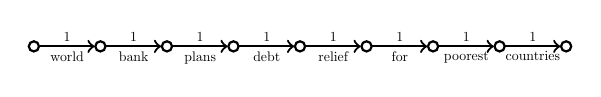
\begin{tikzpicture}[scale=0.65,
nod_s/.style = {scale=0.65, align=center, inner sep=2pt, text centered, circle, draw},
nod_m/.style = {nod_s, thick},
edge_ls/.style = {scale=0.5},
edge_lm/.style = {edge_ls, thick},
edge_ts/.style = {scale=0.5},
edge_tm/.style = {edge_ts},
]

%\newlength{\myx}
%\newlength{\myy}

\setlength{\myx}{1.3cm}
\setlength{\myy}{1.2cm}

\node(0) [nod_m] at (0\myx,0\myy) {};
\node(1) [nod_m] at (1\myx,0\myy) {};
\node(3) [nod_m] at (2\myx,0\myy) {};
\node(4) [nod_m] at (3\myx,0\myy) {};
\node(7) [nod_m] at (4\myx,0\myy) {};
\node(14) [nod_m] at (5\myx,0\myy) {};
\node(20) [nod_m] at (6\myx,0\myy) {};;
\node(27) [nod_m] at (7\myx,0\myy) {};
\node(35) [nod_m] at (8\myx,0\myy) {};

\draw[->,edge_lm] (0) to node [midway, sloped, below, edge_tm] {world\vphantom{pt}} node [midway, sloped, above, edge_tm] {1} (1);
\draw[->,edge_lm] (1) to node [midway, sloped, below, edge_tm] {bank\vphantom{pt}} node [midway, sloped, above, edge_tm] {1} (3);
\draw[->,edge_lm] (3) to node [midway, sloped, below, edge_tm] {plans\vphantom{pt}} node [midway, sloped, above, edge_tm] {1} (4);
\draw[->,edge_lm] (4) to node [midway, sloped, below, edge_tm] {debt\vphantom{pt}} node [midway, sloped, above, edge_tm] {1} (7);
\draw[->,edge_lm] (7) to node [midway, sloped, below, edge_tm] {relief\vphantom{pt}} node [midway, sloped, above, edge_tm] {1} (14);
\draw[->,edge_lm] (14) to node [midway, sloped, below, edge_tm] {for\vphantom{pt}} node [midway, sloped, above, edge_tm] {1} (20);
\draw[->,edge_lm] (20) to node [midway, sloped, below, edge_tm] {poorest\vphantom{pt}} node [midway, sloped, above, edge_tm] {1} (27);
\draw[->,edge_lm] (27) to node [midway, sloped, below, edge_tm] {countries\vphantom{pt}} node [midway, sloped, above, edge_tm] {1} (35);

\end{tikzpicture}
}
\caption{Illustration of rule application (a)}
\label{Ia}
\end{figure}

By using \ac{DFS} to traverse the syntax tree, the program first finds out the pattern started from node \emph{VP} with $2$ levels corresponds the left part of the first rule listed above. This indicates the rule is applicable at this location. According to the reordering rule, the order of the three constituents labeled with \emph{VBZ}, \emph{NP} and \emph{PP} should be changed to \emph{PP VBZ NP} with probability $0.18$. Thus part of the sentence is reordered into \emph{for poorest countries plans debt relief}, and the new path with this probability is added to the word lattice.

\begin{figure}
\centering
\subfigure{
\begin{tikzpicture}[scale=0.5,
-,>=stealth',
level/.style={sibling distance = 2cm, level distance = 1.8cm},
level 1/.style={sibling distance=4cm},
level 2/.style={sibling distance=2cm}, 
level 3/.style={sibling distance=4cm}, 
treenode/.style = {scale=0.5, align=center, inner sep=0.5em, text centered, font=\sffamily},
arn_n/.style = {treenode, rectangle, rounded corners=0.75mm, draw=black, thick, fill=blue!20, minimum width=4em, minimum height = 2em},
arn_x/.style = {arn_n, fill=blue!20, minimum height=3em},
edge from parent fork down
]

\node [arn_n] {S}
child{ node [arn_n] {NP}
child{ node [arn_x] {NN\\ world}}
child{ node [arn_x] {NN\\ bank}}}
child{ node [arn_n,fill=red!20] {VP}
child{ node [arn_x,fill=red!40] {VBZ\\ plans}}
child{ node [arn_n,fill=red!20] {NP}
child{ node [arn_n,fill=red!40] {NP}
child{ node [arn_x] {NN\\ debt}}
child{ node [arn_x] {NN\\ relief}}}
child{ node [arn_n,fill=red!40] {PP}
child{ node [arn_x] {IN\\ for}}
child{ node [arn_n] {NP}
child{ node [arn_x] {JJS\\ poorest}}
child{ node [arn_x] {NNS\\ countries}}}}}};


\end{tikzpicture}


}
\subfigure{
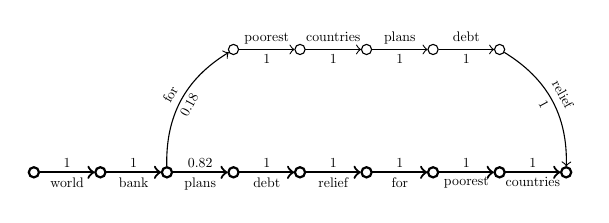
\begin{tikzpicture}[scale=0.65,
nod_s/.style = {scale=0.65, align=center, inner sep=2pt, text centered, circle, draw},
nod_m/.style = {nod_s, thick},
edge_ls/.style = {scale=0.5},
edge_lm/.style = {edge_ls, thick},
edge_ts/.style = {scale=0.5},
edge_tm/.style = {edge_ts},
]

%\newlength{\myx}
%\newlength{\myy}

\setlength{\myx}{1.3cm}
\setlength{\myy}{1.2cm}

\node(0) [nod_m] at (0\myx,0\myy) {};
\node(1) [nod_m] at (1\myx,0\myy) {};
\node(3) [nod_m] at (2\myx,0\myy) {};
\node(4) [nod_m] at (3\myx,0\myy) {};
\node(6) [nod_s] at (3\myx,2\myy) {};
\node(7) [nod_m] at (4\myx,0\myy) {};
\node(13) [nod_s] at (4\myx,2\myy) {};
\node(14) [nod_m] at (5\myx,0\myy) {};
\node(19) [nod_s] at (5\myx,2\myy) {};
\node(20) [nod_m] at (6\myx,0\myy) {};
\node(26) [nod_s] at (6\myx,2\myy) {};
\node(27) [nod_m] at (7\myx,0\myy) {};
\node(34) [nod_s] at (7\myx,2\myy) {};
\node(35) [nod_m] at (8\myx,0\myy) {};

\draw[->,edge_lm] (0) to node [midway, sloped, below, edge_tm] {world\vphantom{pt}} node [midway, sloped, above, edge_tm] {1} (1);
\draw[->,edge_lm] (1) to node [midway, sloped, below, edge_tm] {bank\vphantom{pt}} node [midway, sloped, above, edge_tm] {1} (3);
\draw[->,edge_lm] (3) to node [midway, sloped, below, edge_tm] {plans\vphantom{pt}} node [midway, sloped, above, edge_tm] {0.82} (4);
\draw[->,edge_ls] (3) to [bend left] node [midway, sloped, above, edge_ts] {for\vphantom{pt}} node [midway, sloped, below, edge_ts] {0.18} (6);
\draw[->,edge_lm] (4) to node [midway, sloped, below, edge_tm] {debt\vphantom{pt}} node [midway, sloped, above, edge_tm] {1} (7);
\draw[->,edge_ls] (6) to node [midway, sloped, above, edge_ts] {poorest\vphantom{pt}} node [midway, sloped, below, edge_tm] {1} (13);
\draw[->,edge_lm] (7) to node [midway, sloped, below, edge_tm] {relief\vphantom{pt}} node [midway, sloped, above, edge_tm] {1} (14);
\draw[->,edge_ls] (13) to node [midway, sloped, above, edge_ts] {countries\vphantom{pt}} node [midway, sloped, below, edge_tm] {1} (19);
\draw[->,edge_lm] (14) to node [midway, sloped, below, edge_tm] {for\vphantom{pt}} node [midway, sloped, above, edge_tm] {1} (20);
\draw[->,edge_ls] (19) to node [midway, sloped, above, edge_ts] {plans\vphantom{pt}} node [midway, sloped, below, edge_tm] {1} (26);
\draw[->,edge_lm] (20) to node [midway, sloped, below, edge_tm] {poorest\vphantom{pt}} node [midway, sloped, above, edge_tm] {1} (27);
\draw[->,edge_ls] (26) to node [midway, sloped, above, edge_ts] {debt\vphantom{pt}} node [midway, sloped, below, edge_tm] {1} (34);
\draw[->,edge_lm] (27) to node [midway, sloped, below, edge_tm] {countries\vphantom{pt}} node [midway, sloped, above, edge_tm] {1} (35);
\draw[->,edge_ls] (34) to [bend left] node [midway, sloped, above,  edge_ts] {relief\vphantom{pt}} node [midway, sloped, below, edge_tm] {1} (35);

\end{tikzpicture}
}
\caption{Illustration of rule application (b)}
\end{figure}

As the program keeps running, the second rule is found applicable at another node labeled with \emph{NP} with $2$ levels. Again the rule is applied with probability $0.17$ and the new path is added. 

This illustration uses indices for the reordering rules to avoid ambiguity. The nodes colored with red indicate the part of the syntax tree where a rule is applicable. And the nodes colored with dark red indicate the nodes which are reordered.

\begin{figure}[H]
\centering
\subfigure{
\begin{tikzpicture}[scale=0.5,
-,>=stealth',
level/.style={sibling distance = 2cm, level distance = 1.8cm},
level 1/.style={sibling distance=4cm},
level 2/.style={sibling distance=2cm}, 
level 3/.style={sibling distance=4cm}, 
treenode/.style = {scale=0.5, align=center, inner sep=0.5em, text centered, font=\sffamily},
arn_n/.style = {treenode, rectangle, rounded corners=0.75mm, draw=black, thick, fill=blue!20, minimum width=4em, minimum height = 2em},
arn_x/.style = {arn_n, fill=blue!20, minimum height=3em},
edge from parent fork down
]

\node [arn_n] {S}
child{ node [arn_n] {NP}
child{ node [arn_x] {NN\\ world}}
child{ node [arn_x] {NN\\ bank}}}
child{ node [arn_n] {VP}
child{ node [arn_x] {VBZ\\ plans}}
child{ node [arn_n,fill=red!20] {NP}
child{ node [arn_n,fill=red!20] {NP}
child{ node [arn_x,fill=red!40] {NN\\ debt}}
child{ node [arn_x,fill=red!40] {NN\\ relief}}}
child{ node [arn_n,fill=red!20] {PP}
child{ node [arn_x,fill=red!40] {IN\\ for}}
child{ node [arn_n,fill=red!40] {NP}
child{ node [arn_x] {JJS\\ poorest}}
child{ node [arn_x] {NNS\\ countries}}}}}};


\end{tikzpicture}


}
\subfigure{
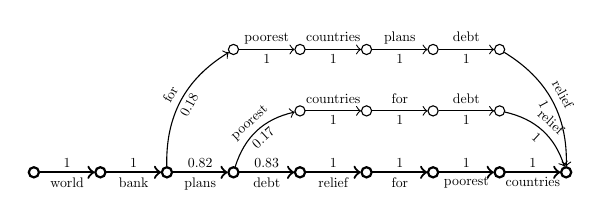
\begin{tikzpicture}[scale=0.65,
nod_s/.style = {scale=0.65, align=center, inner sep=2pt, text centered, circle, draw},
nod_m/.style = {nod_s, thick},
edge_ls/.style = {scale=0.5},
edge_lm/.style = {edge_ls, thick},
edge_ts/.style = {scale=0.5},
edge_tm/.style = {edge_ts},
]

%\newlength{\myx}
%\newlength{\myy}

\setlength{\myx}{1.3cm}
\setlength{\myy}{1.2cm}

\node(0) [nod_m] at (0\myx,0\myy) {};
\node(1) [nod_m] at (1\myx,0\myy) {};
\node(3) [nod_m] at (2\myx,0\myy) {};
\node(4) [nod_m] at (3\myx,0\myy) {};
\node(6) [nod_s] at (3\myx,2\myy) {};
\node(7) [nod_m] at (4\myx,0\myy) {};
\node(11) [nod_s] at (4\myx,1\myy) {};
\node(13) [nod_s] at (4\myx,2\myy) {};
\node(14) [nod_m] at (5\myx,0\myy) {};
\node(17) [nod_s] at (5\myx,1\myy) {};
\node(19) [nod_s] at (5\myx,2\myy) {};
\node(20) [nod_m] at (6\myx,0\myy) {};
\node(24) [nod_s] at (6\myx,1\myy) {};
\node(26) [nod_s] at (6\myx,2\myy) {};
\node(27) [nod_m] at (7\myx,0\myy) {};
\node(32) [nod_s] at (7\myx,1\myy) {};
\node(34) [nod_s] at (7\myx,2\myy) {};
\node(35) [nod_m] at (8\myx,0\myy) {};

\draw[->,edge_lm] (0) to node [midway, sloped, below, edge_tm] {world\vphantom{pt}} node [midway, sloped, above, edge_tm] {1} (1);
\draw[->,edge_lm] (1) to node [midway, sloped, below, edge_tm] {bank\vphantom{pt}} node [midway, sloped, above, edge_tm] {1} (3);
\draw[->,edge_lm] (3) to node [midway, sloped, below, edge_tm] {plans\vphantom{pt}} node [midway, sloped, above, edge_tm] {0.82} (4);
\draw[->,edge_ls] (3) to [bend left] node [midway, sloped, above, edge_ts] {for\vphantom{pt}} node [midway, sloped, below, edge_ts] {0.18} (6);
\draw[->,edge_lm] (4) to node [midway, sloped, below, edge_tm] {debt\vphantom{pt}} node [midway, sloped, above, edge_tm] {0.83} (7);
\draw[->,edge_ls] (4) to [bend left] node [midway, sloped, above, edge_ts] {poorest\vphantom{pt}} node [midway, sloped, below, edge_ts] {0.17} (11);
\draw[->,edge_ls] (6) to node [midway, sloped, above, edge_ts] {poorest\vphantom{pt}} node [midway, sloped, below, edge_tm] {1} (13);
\draw[->,edge_lm] (7) to node [midway, sloped, below, edge_tm] {relief\vphantom{pt}} node [midway, sloped, above, edge_tm] {1} (14);
\draw[->,edge_ls] (11) to node [midway, sloped, above, edge_ts] {countries\vphantom{pt}} node [midway, sloped, below, edge_tm] {1} (17);
\draw[->,edge_ls] (13) to node [midway, sloped, above, edge_ts] {countries\vphantom{pt}} node [midway, sloped, below, edge_tm] {1} (19);
\draw[->,edge_lm] (14) to node [midway, sloped, below, edge_tm] {for\vphantom{pt}} node [midway, sloped, above, edge_tm] {1} (20);
\draw[->,edge_ls] (17) to node [midway, sloped, above, edge_ts] {for\vphantom{pt}} node [midway, sloped, below, edge_tm] {1} (24);
\draw[->,edge_ls] (19) to node [midway, sloped, above, edge_ts] {plans\vphantom{pt}} node [midway, sloped, below, edge_tm] {1} (26);
\draw[->,edge_lm] (20) to node [midway, sloped, below, edge_tm] {poorest\vphantom{pt}} node [midway, sloped, above, edge_tm] {1} (27);
\draw[->,edge_ls] (24) to node [midway, sloped, above, edge_ts] {debt\vphantom{pt}} node [midway, sloped, below, edge_tm] {1} (32);
\draw[->,edge_ls] (26) to node [midway, sloped, above, edge_ts] {debt\vphantom{pt}} node [midway, sloped, below, edge_tm] {1} (34);
\draw[->,edge_lm] (27) to node [midway, sloped, below, edge_tm] {countries\vphantom{pt}} node [midway, sloped, above, edge_tm] {1} (35);
\draw[->,edge_ls] (32) to [bend left] node [midway, sloped, above,  edge_ts] {relief\vphantom{pt}} node [midway, sloped, below, edge_tm] {1} (35);
\draw[->,edge_ls] (34) to [bend left] node [midway, sloped, above,  edge_ts] {relief\vphantom{pt}} node [midway, sloped, below, edge_tm] {1} (35);

\end{tikzpicture}
}
\caption{Illustration of rule application (c)}
\end{figure}

\section{Summary}
In this chapter, we've presented the differences in word orders between English and Chinese, followed by an introduction of the \ac{MLT} reordering algorithm. Because of the different origins and separate development of English and Chinese, they have very distinct sentence structures. To adjust the word order in one language to the other as preordering for translation between the two. It often involves long-distance position change and reordering on multiple level of the syntactic structure. Inspired by the method of tree rules based reordering method, we created the \ac{MLT} reordering algorithm which rearranges the words as a pre-process for translation. The algorithm uses the information of syntactic tree and word alignment, it extracts and applies the reordering rules by detecting patterns from the subtrees with different search levels in syntax trees.
